\providecommand{\main}{../main}
\documentclass[\main/main.tex]{subfiles}
\graphicspath{{../images/}}
\begin{document}
\section{
    ユニタリティ
}
\subsection{
    Euclid空間における共役
}
量子論において重要な性質としてHermite性があるが、これがEuclid空間においてどのように現れるのかを見る。
まずHamiltonianについて、Hermite性
\begin{align}
    \^H^† = \^H
\end{align}
が成り立つことを仮定する。
これは量子論では時間発展がユニタリであることを意味し、統計力学では転送行列がHermiteであることを意味する。
Minkowski時空では、Heisenberg表示の演算子は
\begin{align}
    \^𝒪_\rm{L}(t_\rm{L},𝒙)
    =\e^{\i\^Ht_\rm{L}}\^𝒪_\rm{L}(0,𝒙)\e^{-\i\^Ht_\rm{L}}
\end{align}
と定義される。
この式はMinkowski時空におけるWard-Takahashi恒等式
\begin{align}
    η_{μν}∂^μJ_a^ν𝒪_\rm{L}(x) = \i 𝒬_a 𝒪_\rm{L}(x),
\end{align}
から導くことができる。
ここで$η_{μν}$は符号$(-,+,…,+)$をもつMinkowski計量である。
$𝒪_\rm{L}(0,𝒙)$がHermite演算子であるとき、
\begin{align}
    \^𝒪_\rm{L}(t_\rm{L},𝒙)^†
    =\e^{\i\^Ht_\rm{L}}\^𝒪_\rm{L}(0,𝒙)\e^{-\i\^Ht_\rm{L}}
    = \^𝒪_\rm{L}(t_\rm{L},𝒙)
\end{align}
が成り立つ。
これは量子論で親しんでいる内容である。
次に、これをWick回転した式は
\begin{align}
    \^𝒪_\rm{E}(t_\rm{E},𝒙)
    = \e^{\^Ht_\rm{E}}\^𝒪_\rm{L}(0,𝒙)\e^{-\^Ht_\rm{E}}
\end{align}
となる。
ここで$𝒪_\rm{L}(0,𝒙)$と書いて添字$\rm{E}$ではなく$\rm{L}$をつけているが、Schr\"odinger表示の演算子がWick回転によって不変であることを課して$\^𝒪_\rm{E}(t_\rm{E},𝒙)$を定義している。
この共役は$\^𝒪_\rm{L}(0,𝒙)$がHermiteなとき
\begin{align}\tcboxmath{
    \^𝒪_\rm{E}(t_\rm{E},𝒙)^†
    % = \e^{-\^Ht_\rm{E}}\^𝒪_\rm{L}(0,𝒙)\e^{\^Ht_\rm{E}}
    = \^𝒪_\rm{E}(-t_\rm{E},𝒙)
    \label{QFT: Hermite condition in Euclid spacetime}
}\end{align}
となる。この式がEuclid空間における(Heisenberg表示の演算子に対する)Hermite性の定義である。
ただし、時間成分の添字をもつ演算子の場合は
\begin{align}
    𝒪^0_\rm{E}(0,𝒙) = -\i 𝒪^0_\rm{L}(0,𝒙)
\end{align}
と定義する。
これにより、(\ref{QFT: Hermite condition in Euclid spacetime})の符号が変わる。
同様に、時間の添字が$n$個ある場合は$(-\i)^n$を掛ける。
したがって、テンソル演算子に対し、
\begin{gather}
    𝒪^{μ_1⋯μ_l}_\rm{E}(t,𝒙)^†
    = {Θ^{μ_1}}_{ν_1}⋯{Θ^{μ_l}}_{ν_l}𝒪^{ν_1⋯ν_l}_\rm{E}(-t,𝒙)
    \\
    {Θ^μ}_ν = δ^μ_ν - 2δ^μ_0 δ^0_ν
\end{gather}
が成り立つ。

同様に、状態に対する共役を構成する。
Heisenberg表示の状態は
\begin{align}
    |φ(t)⟩ = \^U(0,t)|φ⟩ = \e^{\^Ht}|φ⟩,
    \␣
    ⟨φ(t)| = ⟨φ|\^U(t,0) = ⟨φ|\e^{-\^Ht}
\end{align}
と定義される。
$|φ(t)⟩$の共役をとると
\begin{align}\tcboxmath{
    |φ(t)⟩^† = ⟨φ|\e^{\^Ht} = ⟨φ(-t)|
}\end{align}
となる。この場合も共役は(Heisenberg表示において)時間反転を伴う。
したがってHermite演算子$\^𝒪(t,𝒙)$に対し、
\begin{align}
    ⟨φ_\rm{f}(t_\rm{f})|\^𝒪(t,𝒙)|φ_\rm{i}(t_\rm{i})⟩^*
    = ⟨φ_\rm{i}(-t_\rm{i})|\^𝒪(-t,𝒙)|φ_\rm{f}(-t_\rm{f})⟩
    \label{conjugate of states}
\end{align}
が成り立つ。
\begin{figure}[H]
    \centering
    
\includegraphics[width=0.5\hsize]{../images/reflection conjugate.pdf}
    \caption{Euclid空間における共役}
\end{figure}
% \begin{align}
%     ⟨ϕ_\rm{f}(t_\rm{f})|𝒪_1(t_1)⋯𝒪_n(t_n)|ϕ_\rm{i}(t_\rm{i})⟩
%     = ⟨ϕ_\rm{i}(-t_\rm{i})|𝒪_n(-t_n)⋯𝒪_1(-t_1)|ϕ_\rm{f}(-t_\rm{f})⟩^*
% \end{align}

\subsection{
    動径量子化における共役
}
次に動径量子化での共役を考える。
共役はHilbert空間に付随する概念なので、量子化の方法(Hilbert空間の取り方)に依存することに注意する。
動径量子化の共役と正準量子化の共役は別の操作であり、同じ記号$†$を用いるが、文脈によって区別してほしい。

動径量子化ではスケール変換の生成子$\^D$がHamiltonianに対応するので、
\begin{align}
    \^D^† = \^D
\end{align}
を仮定する。
これは$\^H$のHermite性より幾分か非自明であるが、シリンダー時空での時間発展のユニタリ性を意味している。
またこの仮定は共形次元が実数となることを保証する。
シリンダー時空の演算子のHermite性は
\begin{align}\tcboxmath{
    \^𝒪(τ,𝒏)^† = \^𝒪(-τ,𝒏), \␣
    \^𝒪(x)^† = \^𝒪\Q(\f{x}{r^2})
}\end{align}
と定義される。
右辺は$𝒪(x)$に対し反転$I: x^μ → x^μ/r^2$を作用させたものになっている。
テンソル演算子の場合、$τ$成分の添字に対して符号を反転させて、
\begin{gather}
    \^𝒪^{μ_1⋯μ_l}(x)^†
    = {I^{μ_1}}_{ν_1}(x)⋯{I^{μ_l}}_{ν_l}(x)
    \^𝒪^{ν_1⋯ν_l}\Q(\f{x}{r^2}),
    \label{tensor radial conjugation}
    \\
    {I^μ}_ν(x) = δ^μ_ν - 2n^μn_ν
    = δ^μ_ν - \f{2x^μx_ν}{r^2}
\end{gather}
となる。

次に、トポロジカル演算子の共役を調べる。
半径$r$の超球面上で積分された運動量は
\begin{align}
    P_μ
    = - r^{d-1}∫\dΩn_ν{T^ν}_μ(x)
\end{align}
と書かれる。
ここで$\dΩ$は極座標の測度を表す。
これを演算子にする場合、
\begin{align}
    P_μ → r^{-1}\^P_μ,\␣
    {T^ν}_μ → r^{-d}\^T^ν{}_μ
\end{align}
として
\begin{align}
    \^P_μ  = -∫\dΩ n_ν\^T^ν{}_μ(n)
\end{align}
となる。ここで$x^μ = rn^μ$とおいている。
同様の議論から
\begin{align}
    \^K_μ = ∫\dΩ n_ν(δ_{μρ}-2n_μn_ρ)\^T_\rm{c}^{νρ}(rn)
\end{align}
となる。
$\^P_μ$の共役をとると、(\ref{tensor radial conjugation})を用いて
\begin{align}
    \^P_μ^†
    = ∫\dΩ n_ν(δ_{μρ} - 2n_μn_ρ)\^T^{νρ}\Q(\f{n}{r})
    = \^K^μ
\end{align}
を得る。
角運動量演算子に対しては、
\begin{align}
    \^M_{μν}
    = -∫\dΩ n_ρ (n_ν\^T^ρ{}_μ-n_μ\^T^ρ{}_ν)
\end{align}
から、
\begin{align}
    \^M_{μν}^†
    &
    = ∫\dΩ n_ρ (-n_ν\^T^ρ{}_σ(δ^σ_μ-2n^σn_μ)+n_μ\^T^ρ{}_σ(δ^σ_ν-2n^σn_ν))
    \∅ &
    = -\^M_{μν}^†
\end{align}
となる。
以上をまとめて、
\begin{align}\tcboxmath{
    \^P_μ^† = \^K_μ,\␣
    \^K_μ^† = \^P_μ,\␣
    \^M_{μν}^† = -\^M_{μν}
    \label{radial conjugation of topological operators}
}\end{align}
となる。これらの式は以下の方法によっても導出可能である。
\footnote{
    動径量子化の共役が反転を表すことから生成子の両側に$I$を掛ける。負号がつくのは量子力学で$\∂*{x}^† = -\∂*{x}$とするのと同じ理由で、部分積分をすることによる。
}
\begin{align}
    P_μ^† ≔ -IP_μI = K_μ,\␣
    M_{μν}^† ≔ -IM_{μν}I = -M_{μν}
\end{align}
$I$は反転変換を表す。
また、(\ref{radial conjugation of topological operators})は交換関係
\begin{align}
    [D,P_μ] = P_μ,\␣
    [D,K_μ] = K_μ
\end{align}
と整合する。

\subsection{
    ユニタリティと鏡映正値性
}
我々が通常興味のある場の量子論は、ユニタリな理論である。
これは状態空間が正定値の内積をもつと言い換えられる。
% \footnote{
%     補助場を考える場合に正定値ではない状態空間を扱う場合があるが、それは計算上の便宜のためであって、物理的な場から構成した状態空間は基本的にユニタリである。
% }
Euclid空間の場の理論においてユニタリティに対応する概念は鏡映正値性(reflection positivity)と呼ばれる性質である。
Euclid空間での状態を
\begin{align}
    \^𝒪₁(-t₁)⋯\^𝒪ₙ(-tₙ)|0⟩,\␣
    (-t₁>⋯>-tₙ)
\end{align}
と書くと、その共役は
\begin{align}
    ⟨0|\^𝒪ₙ(tₙ)⋯\^𝒪₁(t₁)
\end{align}
で与えられる。
ただし(\ref{QFT: Hermite condition in Euclid spacetime})を仮定した。
状態空間の正定値性は
\begin{align}
    ⟨0|\^𝒪ₙ(tₙ)⋯\^𝒪₁(t₁)\^𝒪₁(-t₁)⋯\^𝒪ₙ(-tₙ)|0⟩
    ≥ 0
\end{align}
と書ける。相関関数で書くと
\begin{align}
    \⟨𝒪ₙ(tₙ)⋯𝒪₁(t₁)𝒪₁(-t₁)⋯𝒪ₙ(-tₙ)\⟩ ≥ 0
\end{align}
となる。この性質を\textbf{鏡映正値性(reflection positivity)}という。

\begin{figure}[H]
    \centering
    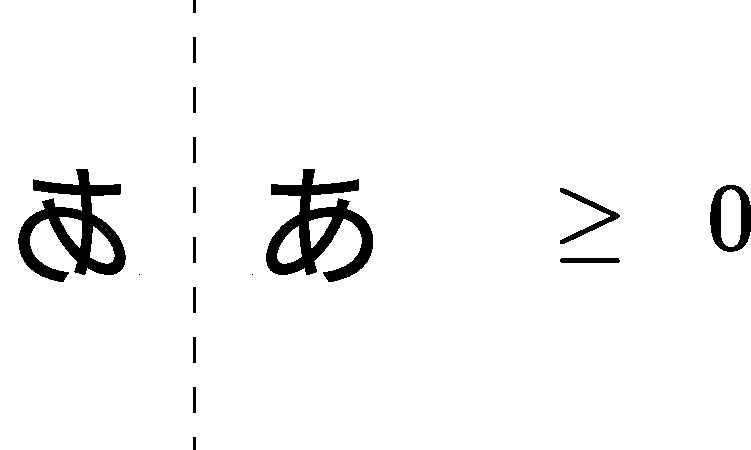
\includegraphics[width=0.25\hsize]{../images/reflection positivity.pdf}
    \caption{鏡映正値性}
\end{figure}
動径量子化についての鏡映正値性は
\begin{align}
    \⟨𝒪ₙ(τₙ)⋯𝒪₁(τ₁)𝒪₁(-τ₁)⋯𝒪ₙ(-τₙ)\⟩ ≥ 0
\end{align}
となる。
\subsection{
    ユニタリティバウンド
}
用いる交換関係を以下に載せておく。
\begin{align*}
    &
    [K_μ,P_ν] = 2δ_{μν}D - 2M_{μν}
    \\ &
    [D, P_μ] = P_μ
    \\ &
    [M_{νρ},P_σ] = -δ_{νσ}P_ρ + δ_{ρσ}P_ν
\end{align*}
動径量子化におけるユニタリティ(鏡映正値性)を仮定して共形次元に対する制限を導く。
まず、スカラープライマリー状態$|𝒪⟩$に対し、
\begin{align}
    ⟨𝒪|𝒪⟩ ≥ 0
\end{align}
が成り立つ。
次にレベル1のディセンダント状態について考える。
交換関係を用いると、
\begin{align}
    ⟨𝒪|K_μP_ν|𝒪⟩
    &
    = ⟨𝒪|(P_νK_μ+2δ_{μν}D-2M_{μν})|𝒪⟩
    \∅ &
    = 2Δδ_{μν}⟨𝒪|𝒪⟩
\end{align}
となり、ユニタリティから$Δ ≥ 0$が分かる。

また$Δ=0$の場合、$‖P_μ|𝒪⟩‖=0$となることから、ユニタリな理論では$P_μ|𝒪⟩=0$となる。
したがって$|𝒪⟩$真空状態となり、対応する演算子$𝒪(x)$は$x$に依存しない恒等演算子となる。

次にレベル2のディセンダント状態について
\begin{align}
    ⟨𝒪|K_μK_νP_ρP_σ|𝒪⟩
    = ⟨𝒪|K_μP_ρK_νP_σ|𝒪⟩
    + 2⟨𝒪|K_μ(δ_{νρ}D-M_{νρ})P_σ|𝒪⟩
\end{align}
となる。各項は
\begin{gather}
    ⟨𝒪|K_μP_ρK_νP_σ|𝒪⟩
    = 4Δ^2δ_{μρ}δ_{νσ}
    \\
    2δ_{νρ}⟨𝒪|K_μDP_σ|𝒪⟩
    = 4(Δ^2+Δ)δ_{μσ}δ_{νρ}
    \\
    -2⟨𝒪|K_μM_{νρ}P_σ|𝒪⟩
    = 4Δδ_{νσ}δ_{μρ} - 4Δδ_{ρσ}δ_{μν}
\end{gather}
と計算されるので、
\begin{align}
    ⟨𝒪|K_μK_νP_ρP_σ|𝒪⟩
    = 4Δ(Δ+1)(δ_{μρ}δ_{νσ}+δ_{μσ}δ_{νρ})
    -4Δδ_{μν}δ_{ρσ}
\end{align}
を得る。
$P_μP_ν|𝒪⟩$を回転に対する既約表現に分解して考えるのが最も一般的な議論だが、ここでは$P^2|𝒪⟩$についてのユニタリティバウンドを考える。
これは$μ=ν,ρ=σ$として縮約をとれば良いので、
\begin{align}
    8Δ(Δ+1)d - 4Δd^2 ≥ 0
\end{align}
が得られる。$Δ ≥ 0, d > 0$から
\begin{align}\tcboxmath{
    Δ ≥ \f{d}{2} -1
}\end{align}
となる。
同様の議論をもっと高いレベルのディセンダントで行うこともできるが、これ以上厳しい条件は出てこないことが知られている。

\subsection{
    スピンを持つ演算子のユニタリティバウンド
}
スピンを持つ演算子についてもユニタリティから共形次元に対する不等式を導くことができる。
まず、プライマリー状態の規格化を
\begin{align}
    ⟨𝒪^a|𝒪_b⟩ = δ^a_b
\end{align}
とする。
レベル1のディセンダントについて、
\begin{align}
    ⟨𝒪^a|K_μP_ν|𝒪_b⟩
    = 2Δδ_{μν}δ^a_b - 2{(𝒮_{μν})_a}^b
\end{align}
となる。
ユニタリティから右辺の行列の固有値は全て非負になる必要があるので、
\begin{align}
    Δ ≥ \t{max-eigenvalue}\,({(𝒮_{μν})_a}^b)
    \label{level 1 unitarity bound with spin}
\end{align}
が言える。ここで、
\begin{align}
    &
    {(𝒮_{μν})_a}^b
    = \f{1}{2}(L^{αβ})_{μν}{(𝒮_{αβ})_a}^b,
    \∅ &
    (L^{αβ})_{μν} = δ^α_μδ^β_ν - δ^α_νδ^β_μ
\end{align}
と書く。
$αβ = A$と書き、$(L^A)_{μν},{(𝒮_A)_a}^b$を表現空間$V,R_𝒪$に対する$M^A$の表現とみなすと、
\begin{align}
    𝒮 = L^A 𝒮_A
    &
    = \f{1}{2}((L+𝒮)^2 - L^2 - 𝒮^2)
    \∅ &
    = \f{1}{2}(
        -\rm{Cas}(V⊗R_𝒪)
        +\rm{Cas}(V)
        +\rm{Cas}(R_𝒪)
    )
\end{align}
と書ける。つまり、$𝒮$をCasimir演算子のみで表すことができる。

以降はスピン$l$のトレースレス演算子の場合を考える。
このとき$R_𝒪$はスピン$l$の既約表現となり、$R_𝒪 = V_l$と書くことにする。
$V ⊗ V_l$は
\begin{align}
    V ⊗ V_l = V_{l-1} ⊕ ⋯ \␣ (l > 0)
\end{align}
と既約分解できる。最もスピンが小さい空間のみが最大固有値に寄与するので、
\begin{align}
    Δ 
    &
    ≥\f{1}{2}(
        -\rm{Cas}(V_{l-1})+\rm{Cas}(V_l)+\rm{Cas}(V)
    )
    \∅ &
    = \f{1}{2}\Q\Big(
        -(l-1)(l+d-3)+l(l+d-2)+(d-1)
    )
\end{align}
と書ける。ここで、$d$次元空間のスピン$l$の状態に対するCasimir演算子の固有値が$\rm{Cas}(V_l) = l(l+d-2)$であることを用いた。
整理して
\begin{align}\tcboxmath{
    Δ ≥ l+d-2
}\end{align}
となる。
もっと高いレベルのディセンダントで同様の議論が可能だが、これ以上厳しい条件は出てこないことが知られている。
\end{document}